%!TEX root=./report.tex
\section{EVALUATION}

\subsection{Evaluation Metrics}
As a reminder, our task is identifying the correct object model from a large database, given a scan of a model in an uncluttered scene.

We evaluate the correctness of our results with the following metrics:
\begin{itemize}
  \item Percentage of ultimate guesses correct
  \item Confusion matrix for ultimate guess
  \item Precision-recall curve (using registration results)
  \item Average rank of correct model (using voting results)
  \item Area under the cumulative result-within-top-K histogram
\end{itemize}

The results for the Princeton Shape Benchmark can be seen in~\ref{tab:psb_results}
\begin{table}
  \centering
  \documentclass[10pt]{article}
\usepackage[usenames]{color} %used for font color
\usepackage{amssymb} %maths
\usepackage{amsmath} %maths
\usepackage[utf8]{inputenc} %useful to type directly diacritic characters
\usepackage{multirow}
\begin{document}

\begin{tabular}{ | l || l | l | l | l | }
\hline
Metric & PFH & FPFH & SHOT & SPIN IMAGE \\
\hline
 \% Correct & 86.25 & 87.50 & 73.75 & 49.35 \\
AP & 0.850 & 0.855 & 0.635 & 0.307 \\
Avg. Rank & 2.250 & 2.160 & 2.300 & 3.960 \\
AUH & 0.844 & 0.855 & 0.838 & 0.654 \\
\hline
\end{tabular}
\end{document}
  \caption{Results on the Princeton Shape Benchmark.}
  \label{tab:psb_results}
\end{table}

%\begin{figure*}
%  \centering
%  \subfloat[]{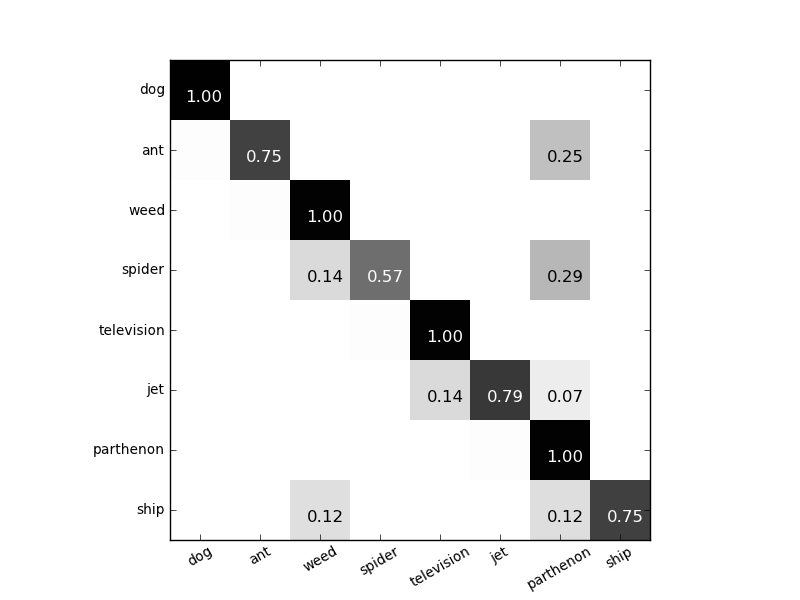
\includegraphics[width=0.45\textwidth]{../figures/PFH_confmat.png}}
%  \subfloat[]{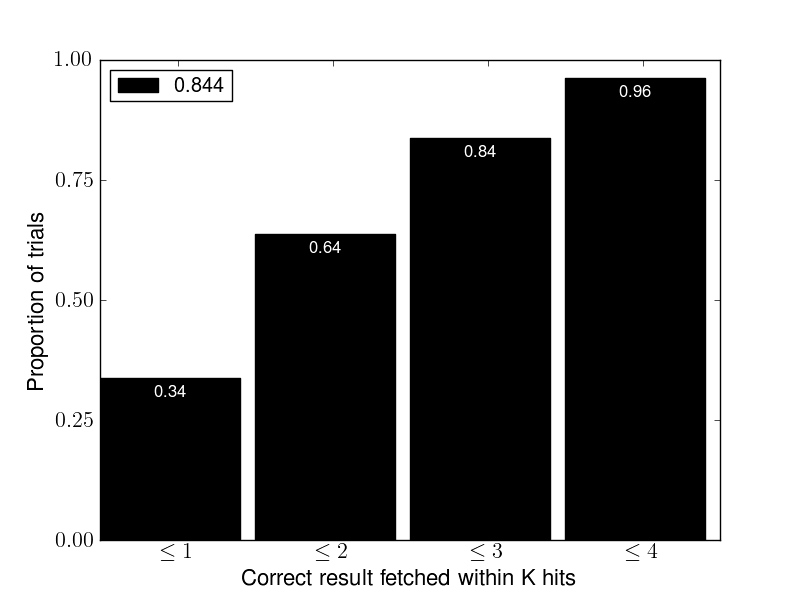
\includegraphics[width=0.45\textwidth]{../figures/PFH_rankhist.png}} \\
%  \subfloat[]{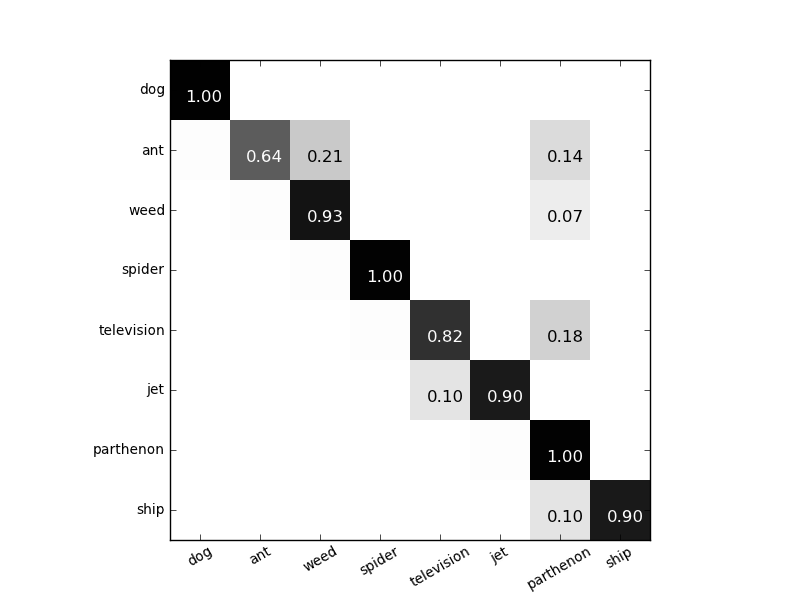
\includegraphics[width=0.45\textwidth]{../figures/FPFH_confmat.png}}
%  \subfloat[]{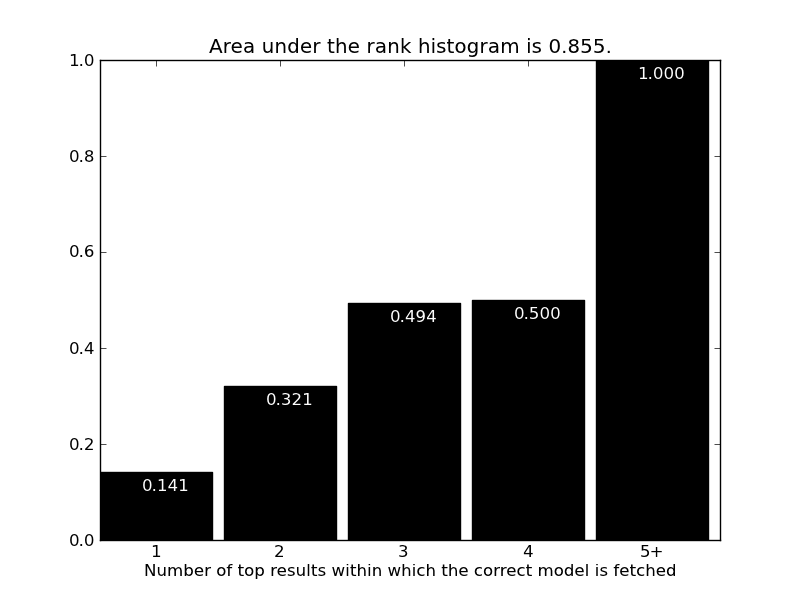
\includegraphics[width=0.45\textwidth]{../figures/FPFH_rankhist.png}} \\
%  \caption{Dashboard figure}
%  \label{fig:animals}
%\end{figure*}

\begin{table*}
\centering
\begin{tabular}{m{0.03\textwidth} m{0.45\textwidth} m{0.45\textwidth}}
     & \begin{center} Confusion Matrix \end{center} & \begin{center} Cumulative Rank Histogram \end{center} \\
  {\large PFH} & 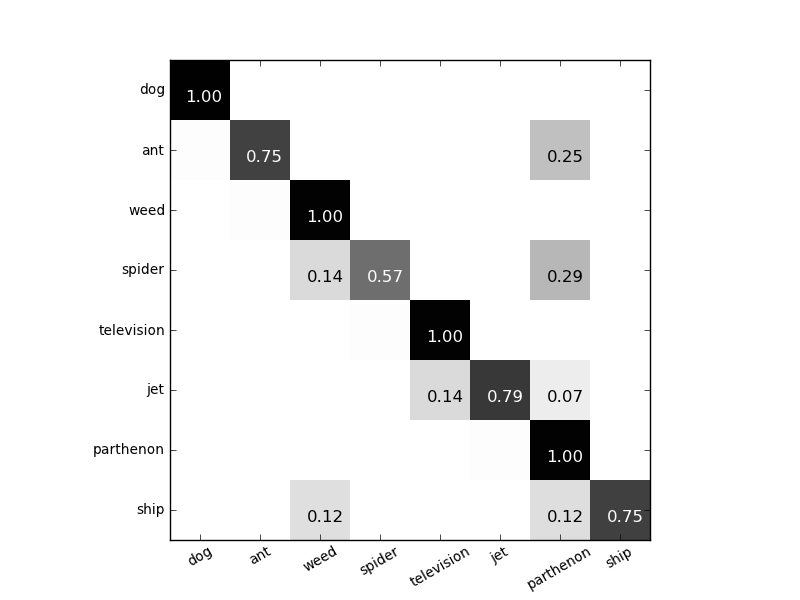
\includegraphics[width=0.45\textwidth,clip=true]{../figures/PFH_confmat.png} & 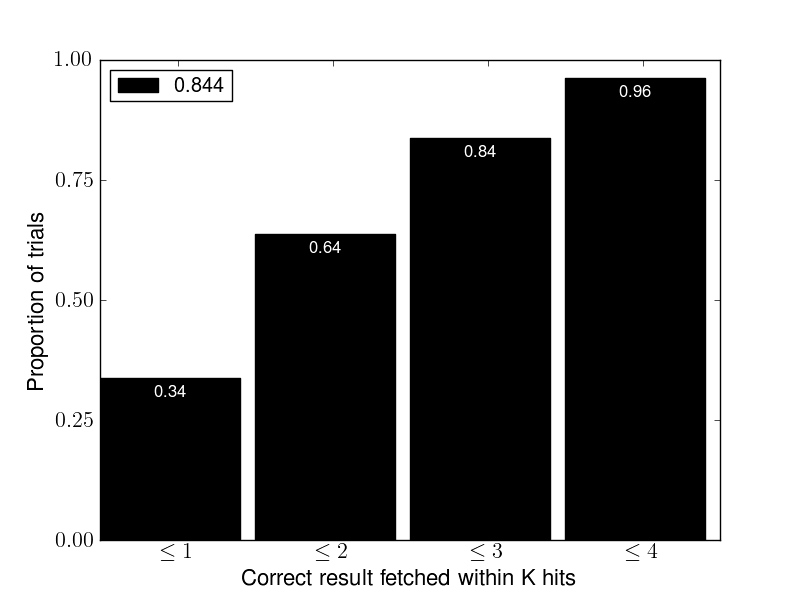
\includegraphics[width=0.45\textwidth,clip=true]{../figures/PFH_rankhist.png} \\
  {\large FPFH} & 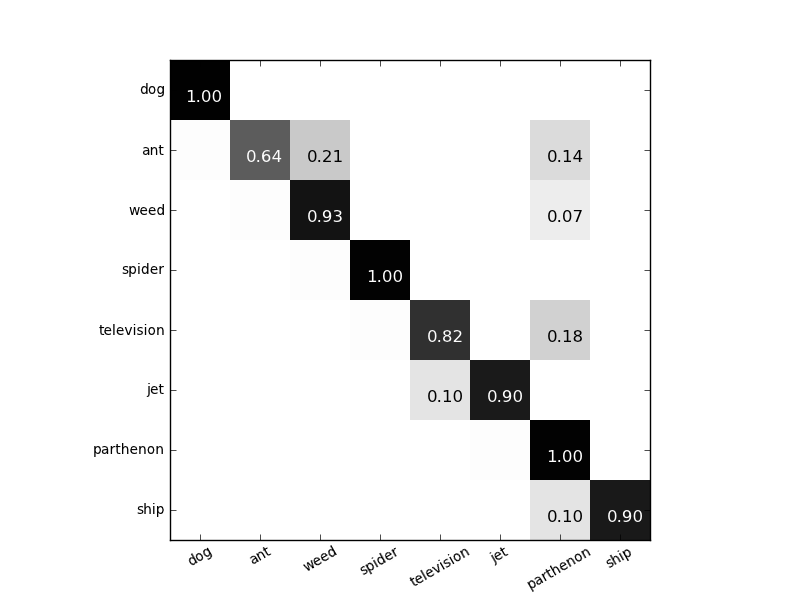
\includegraphics[width=0.45\textwidth,clip=true]{../figures/FPFH_confmat.png} & 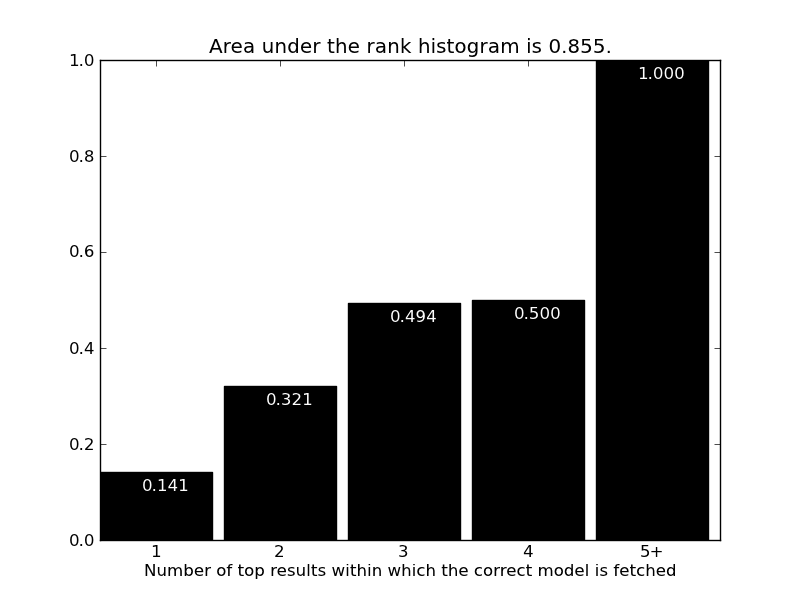
\includegraphics[width=0.45\textwidth,clip=true]{../figures/FPFH_rankhist.png} \\
\end{tabular}
\caption{A table arranging images}
\label{tab:gt}
\end{table*}

An additional important evaluation is the runtime performance of different methods.
This data allows focused work on fast feature extraction and on algorithms to speed up matching, such as locality-sensitive hashing \cite{Frome2004}.
Hence, we report timing results, split by the different stages of our pipeline, for all experimental conditions.
In all cases, the tests were run on a 2.50 GHz Intel Core2 Quad Q9300 with 4 GB of RAM.

* table per dataset

* features vs. metrics

* plots of the same data that's in the tables?

* confusion matrix figures

* table of timing results

%\begin{figure}[thpb]
%   \centering
%   \label{fig:results}
%\end{figure}
